\documentclass[twoside,10pt]{report}
\usepackage{/Users/bradenhoagland/latex/breaks}
\toggletrue{sectionbreaks}
\newcommand{\docTitle}{Topology}
\usepackage{/Users/bradenhoagland/latex/math2}

%\renewcommand{\theenumi}{\alph{enumi}}

\begin{document}
\tableofcontents

%+-------------------+
%| +---------------+ |
%| |    Chapter    | |
%| +---------------+ |
%+-------------------+
% Topological Spaces


\chapter{Topological Spaces}

%%%%%%%%%%%%%%%%%%%%
% Topological Spaces
%%%%%%%%%%%%%%%%%%%%

\section{Topological Spaces}

\begin{defn}
	Let $X$ be a set, then a \textbf{topology} on $X$ is a collection $\mathcal{T}$ of subsets of $X$ such that
	\begin{enumerate}
		\item $\varnothing, X \in \mathcal{T}$,
		\item $\bigcup_{\alpha\in \mathcal{J}}U_\alpha \in \mathcal{T}$, and
		\item $\bigcap_{i=1}^N U_i \in \mathcal{T}$.
	\end{enumerate}
	Elements of a topology are called \textbf{open sets}.
\end{defn}

\begin{ex}
\begin{enumerate}
	\item ``Indiscrete" topology: $\mathcal{T}_i = \left\{ \varnothing, X \right\}$ 
	\item ``Discrete" topology: $\mathcal{T}_d =\{$all subsets of $X\}$
\end{enumerate}
\end{ex}

\begin{defn}
	Let $\mathcal{T},\mathcal{T}'$ be topologies on a set $X$, then $\mathcal{T}$ is \textbf{finer} than $\mathcal{T}'$ if $\mathcal{T}' \subset \mathcal{T}$. $\mathcal{T}$ is \textbf{coarser} than $\mathcal{T}'$ if $\mathcal{T} \subset \mathcal{T}'$. The notions of \textbf{strictly finer} and \textbf{strictly coarser} follow.
\end{defn}

From this we see that ``fine" is a notion of a large topology, and ``coarse" is a notion of a small topology.

\begin{ex}[]
	The \textbf{lower limit topology} on $\mathbb{R}$ is given by the basis
	\[
		\mathcal{B}= \left\{ [a,b) \;|\; a < b \right\}.
	\] It is strictly finer than the standard topology on $\mathbb{R}$: since $\bigcup_{n\in \mathbb{N}}[a + 1/n, b)=(a,b)$, it contains the standard topology, but $[a,b)$ is not open in the standard topology, so it is strictly finer.
\end{ex}

\begin{ex}[]
	Let $X$ be any set, then the \textbf{finite complement topology} is defined
	\[
		\mathcal{T}_f = \left\{ U \subset X \;|\; X-U \text{ is finite} \right\} \cup\left\{ \varnothing \right\},
	\] 
	where $X-U$ denotes the complement of $U$ in $X$, i.e. $X \backslash U$. Checking that this is a topology boils down to just using DeMorgan's Laws.
\end{ex}

%%%%%%%%%%%%%%%%%%%%
% Closed Sets and Limit Points
%%%%%%%%%%%%%%%%%%%%

\section{Closed Sets and Limit Points}

\begin{defn}
	A set $A \subset (X, \mathcal{T})$ is closed if $X-A$ is open in $X$.
\end{defn}

\begin{thrm}
	Let $(X, \mathcal{T})$ be a topological space, and let $F$ denote a closed set of $X$, then
	\begin{enumerate}
		\item $\varnothing$ and $X$ are closed,
		\item $\bigcap_{\alpha\in\mathcal{J}}F_\alpha$ is closed, and
		\item $\bigcup_{i=1}^N F_i$ is closed.
	\end{enumerate}
\end{thrm}
\begin{proof}
This is a straightforward application of DeMorgan's Laws.
\end{proof}

Properties of a closed set $A$ in a subspace $Y$ of $X$:
\begin{itemize}
	\item $A$ is the intersection of $Y$ and a closed set in $X$.
	\item If $Y$ is closed in $X$, then $A$ is closed in $X$.
\end{itemize}

\begin{prop}
Let $Y$ be a subspace of $X$. Then $A$ is closed in $Y$ if and only if it is equal to the intersection of a closed set of $X$ with $Y$.
\end{prop}

\begin{prop}
Let $Y$ be a subspace of $X$. If $A$ is closed in $Y$ and $Y$ is closed in $X$, then $A$ is closed in $X$.
\end{prop}

\begin{defn}
	The \textbf{interior} of a set $A$, denoted $A^o$, is the union of all open sets contained in $A$.

	The \textbf{closure} of a set $A$, denoted $\overline{A}$ is the intersection of all closed sets containing $A$.
\end{defn}

The closure of a set is clearly closed, and the interior of a set is clearly open. It is also clear that if $A$ is open, then $A^o = A$, and if $A$ is closed, then $\overline{A}=A$. We also have the obvious relation $A^o \subset A \subset \overline{A}$.

We have to be careful when describing closures. Given a subspace $Y$ of $X$, the closure of $A$ in $X$ is generally not the same as the closure of $A$ in $Y$. In this case, we use $\overline{A}$ to denote the closure of $A$ in $X$ (the overall space). We relate this to the closure of $A$ in $Y$ (the subspace) with the following proposition.

\begin{prop}
	Let $Y$ be a subspace of $X$, and let $A \subset Y$. Then $\overline{A}_{Y}=\overline{A}_{X} \cap Y$.
\end{prop}

\begin{defn}
A \textbf{neighborhood} of a point $X$ is an open set containing $x$.
\end{defn}

\begin{thrm}
	\label{thrm:nhood-closure}
Let $A$ be a subset of a topological space $X$, then
\begin{enumerate}
	\item $x \in \overline{A}$ if and only if every neighborhood of $x$ intersects $A$, and
	\item Supposing the topology of $X$ is given by a basis, then $x \in \overline{A}$ if and only if every basis element $B$ containing $x$ intersects $A$.
\end{enumerate}
\end{thrm}
{\color{red}Make sure you have an intuitive understanding of why this is true.}

\begin{defn}
Let $A \subset (X,\mathcal{T})$, then $x \in X$ is a \textbf{limit point} of $A$ if every open neighborhood of $x$ intersects $A$ at some point \textit{other than} $x$.

	Equivalently, $x$ belongs to the closure of $A - \left\{ x \right\}$. Note that $x$ need not lie in $A$. {\color{red}Think about this.}
\end{defn}

\begin{thrm}
	Let $A \subset (X,\mathcal{T})$, and denote the set of limit points of $A$ by $A'$. Then $\overline{A}=A \cup A'$.
\end{thrm}

\begin{cor}
	A subset of a topological space is closed if and only if it contains all its limit points.
\end{cor}
\begin{proof}
	Let $A \subset (X, \mathcal{T})$. Then $A$ is closed if and only if $A = \overline{A} = A \cup A'$, and $A = A \cup A'$ if and only if $A' \subset A$.
\end{proof}

%%%%%%%%%%%%%%%%%%%%
% Bases
%%%%%%%%%%%%%%%%%%%%

\section{Bases}

\begin{defn}
Let $\mathcal{T}$ be a topoloy on $X$, and let $\mathcal{B} \subset \mathcal{T}$. Then $\mathcal{B}$ is a \textbf{basis} for $\mathcal{T}$ if every open set of $\mathcal{T}$ can be written as the union of elements of $\mathcal{B}$.
\end{defn}

\begin{prop}
\label{prop:basis-specific-top}
Let $\mathcal{T}$ be a topology on $X$, and let $\mathcal{B}$ be a collection of subsets of $X$. Then $\mathcal{B}$ is a basis for $\mathcal{T}$ if and only if
\begin{enumerate}
	\item $\mathcal{B}\subset \mathcal{T}$; and
	\item for each $U \in \mathcal{T}$ and $p \in U$, there is a $B \in \mathcal{B}$ such that $p \in B \subset U$.
\end{enumerate}
\end{prop}
\begin{proof}
	The forward direction follows from every open set of $\mathcal{T}$ being the union of elements of $\mathcal{B}$. For the backward direction, since $p \in B_p \subset U$ for all $p \in U$, we have $U = \bigcup_{p\in U}B_p$, so every open set of $\mathcal{T}$ is the union of elements of $\mathcal{B}$. 
\end{proof}

\begin{figure}[H]
	\centering
	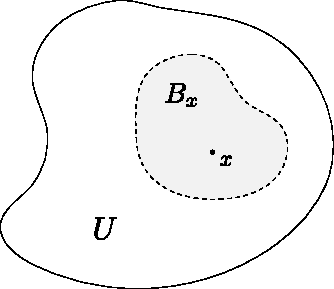
\includegraphics[scale=0.8]{fig/gen-top.pdf}
	\caption{For any $U \in \mathcal{T}$, each $x \in U$ lies in some $B_x \in \mathcal{B}$ for $B_x \subset U$.}
\end{figure}


Not every set of subsets of $X$ will generate a topology, so we need conditions for a collection $\mathcal{B}$ to be a basis for \textit{any} topology.

\begin{prop}
\label{prop:basis-for-any-top}
Let $\mathcal{B}$ be a collection of subsets of $X$. Then $\mathcal{B}$ generates a topology if and only if
\begin{enumerate}
	\item $\bigcup_{B \in \mathcal{B}}=X$.
	\item given $B_1,B_2 \in \mathcal{B}$ and $x \in B_1 \cap B_2$, there is a $B_3 \in \mathcal{B}$ such that $x \in B_3 \subset B_1 \cap B_2$.
\end{enumerate}
\end{prop}
\begin{proof}
	\textbf{Forward:} (1) $X$ must be open, so $X$ is the union of the elements of $\mathcal{B}$. (2) Since $B_1$ and $B_2$ are both open in the topology generated by $\mathcal{B}$, their intersection is, as well. Then since $\mathcal{B}$ is a basis for this topology, we can find a satisfactory $B_3$.

	\textbf{Backward:} The topology generated by a set $\mathcal{B}$ is the collection of all unions of elements of $\mathcal{B}$. It is clear that $\varnothing$ is in it, and condition (1) implies that $X$ is, as well. Arbitrary unions are in the topology by definition. Induction on condition (2) shows that the topology also contains finite intersections.
\end{proof}

\begin{figure}[H]
	\centering
	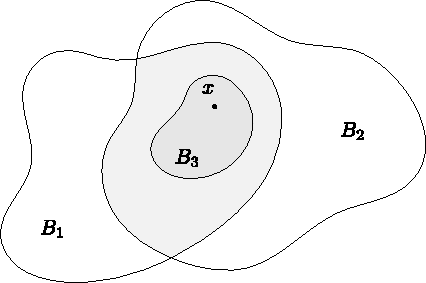
\includegraphics[scale=1]{fig/basis.pdf}
	\caption{Condition $(2)$ in Proposition \ref{prop:basis-for-any-top}.}
\end{figure}

\begin{note}
Since $\mathcal{B}$ exists independently from any topology, it doesn't make sense to describe its members as ``open" until after we've generated a topology from it. Once we've done so, though, it should be clear that every basis element is open in the generated topology.
\end{note}

We can also get a notion of how relatively fine or coarse a topology is by using its basis.

\begin{prop}
	Let $\mathcal{B}, \mathcal{B}'$ be bases for the topologies $\mathcal{T},\mathcal{T}'$ on $X$, respectively. Then $\mathcal{T}'$ is finer than $\mathcal{T}$ if and only if for all $B \in \mathcal{B}$ and $x \in B$, there is a $B' \in \mathcal{B}'$ such that $x \in B' \subset \mathcal{B}$.
\end{prop}
\begin{proof}
	First we show the backward implication. Let $U \in \mathcal{T}$, and let $x \in U$. Since $\mathcal{B}$ generates $\mathcal{T}$, there is a $B \subset \mathcal{B}$ such that $x \in B \subset U$. By assumption, there is then a $B' \in \mathcal{B}'$ such that $x \in B' \subset B \subset U$. Thus $U \in \mathcal{T}'$, so $\mathcal{T}'$ is finer than $\mathcal{T}$.

	Now we show the forward implication. Let $B \in \mathcal{B}$, and let $x \in B$, then $B \in \mathcal{T}$. By assmption, $\mathcal{T} \subset \mathcal{T}'$, so $B \in \mathcal{T}'$ as well. Then by the definition of a generated topology, there is a $B' \subset \mathcal{B}'$ such that $x \in B' \subset B$.
\end{proof}

\begin{prop}
The topology generated by a basis is the smallest topology containing that basis.
\end{prop}

%%%%%%%%%%%%%%%%%%%%
% Subbases
%%%%%%%%%%%%%%%%%%%%

\section{Subbases}

\begin{defn}
	A \textbf{subbasis} $\mathcal{S}$ for a topology $\mathcal{T}$ on $X$ is a collection of subsets of $X$ whose finite intersections form a basis for $\mathcal{T}$.
\end{defn}

Subbases are easier to construct than bases, but the construction of a topology from a subbasis involves an extra step, namely the finite intersections. What we are doing is creating a basis $\mathcal{B}$ from $\mathcal{S}$ by taking finite intersections of the subbasis elements. Then we are taking $\mathcal{B}$ and constructing $\mathcal{T}$ by taking arbitrary unions, as is usual.

\begin{figure}[H]
	\centering
	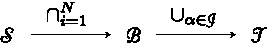
\includegraphics[scale=1]{fig/subbasis-to-topology.pdf}
	\caption{The process for constructing a topology using a subbasis $\mathcal{S}$.}
\end{figure}

\begin{prop}
Let $\mathcal{T}$ be a topology on $X$, and let $\mathcal{S}$ be a collection of subsets of $X$. Then $\mathcal{S}$ is a subbasis for $\mathcal{T}$ if and only if
\begin{enumerate}
	\item $\mathcal{S} \subset \mathcal{T}$; and
	\item for each $U \in \mathcal{T}$ and $p \in U$, there is a finite intersection $\bigcap_{i=1}^n S_i$ of elements of $\mathcal{S}$ such that $p \in \bigcap_{i=1}^n S_i \subset U$.
\end{enumerate}
\end{prop}
\begin{proof}
	This follows from Proposition \ref{prop:basis-specific-top} (the analogue of this proposition for bases). When proving both directions, there's just an extra step to go from a genric basis element to a finite intersection of elements of $\mathcal{S}$.
\end{proof}

\begin{prop}
Let $\mathcal{S}$ be a collection of subsets of $X$. Then $\mathcal{S}$ generates a topology if and only if $\mathcal{S}$ covers $X$.
\end{prop}

\begin{prop}
The topology generated by a subbasis is the smallest topology containing that subbasis.
\end{prop}

%%%%%%%%%%%%%%%%%%%%
% Continuous Functions
%%%%%%%%%%%%%%%%%%%%

\section{Continuous Functions}

The category \cat{Top} has topological spaces as objects and continuous functions as morphisms.

\begin{defn}
	Let $X,Y$ be topological spaces, then $f : X \to Y$ is \textbf{continuous} if for all $U$ open in $Y$, $f^{-1}(U)$ is open in $X$.
\end{defn}

\begin{prop}
	If $Y$ has basis $\mathcal{B}$ and $f^{-1}(B)$ is open in $X$ for all $B \in \mathcal{B}$, then $f: X \to Y$ is continuous.
	Similarly, if $Y$ has subbasis $\mathcal{S}$ and $f^{-1}(S)$ is open in $X$ for all $S \in \mathcal{S}$, then $f: X \to Y$ is continuous.
\end{prop}
\begin{proof}
	The preimage of any open set if the union of preimages of basis elements. The preimage of any basis element is the finite intersection of preimages of subbasis elements.
\end{proof}

\begin{thrm}
Let $X$ and $Y$ be topological spaces, and let $f: X \to Y$, then the following are equivalent:
\begin{enumerate}
	\item $f$ is continuous.
	\item For all $A \subset X$, $f(\overline{A}) \subset \overline{f(A)} $.
	\item For all $B$ closed in $Y$, $\overline{f^{-1}(B)} \subset f^{-1}(\overline{B})$.
	\item For all $B$ closed in $Y$, $f^{-1}(B)$ is closed in $X$.
	\item For all $x \in X$ and for each neighborhood $V$ of $f(x)$, there is a neighborhood $U$ of $x$ such that $f(U) \subset V$.
\end{enumerate}
\end{thrm}

\begin{ex}[]
	If $X$ has the discrete topology, then any function \textit{out} of $X$ is continuous. If $X$ has the indiscrete topology, then any function \textit{into} $X$ is continuous.
\end{ex}

\begin{defn}
	A \textbf{homeomorphism} is a continuous function with continuous inverse (an isomorphism in \cat{Top}).

	Equivalently, a homeomorphism is a bijective function $f: X \leftrightarrow Y$ such that $U$ is open in $X$ if and only if $f(U)$ is open in $Y$.
\end{defn}

\begin{figure}[H]
	\centering
	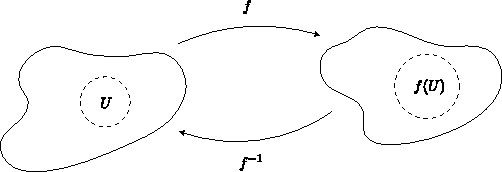
\includegraphics[scale=1.3]{fig/homeomorphism.pdf}
	\caption{A homeomorphism $f$.}
\end{figure}

\begin{thrm}[The Pasting Lemma]
	Let $X = A \cup B$, where $A$ and $B$ are either both closed or both open in $X$. Let $f:A \to Y$ and $g:B\to Y$ be continuous. If $f(x)=g(x)$ for all $x \in A \cap B$, then the function $h : X \to Y$ given by
	\[
		H(x)=
		\begin{cases}
			f(x) & x \in A \\
			g(x) & x\in B
		\end{cases}
	\] is continuous.
\end{thrm}
\begin{proof}
	Suppose $A$ and $B$ are both closed. Let $C$ be closed in $Y$, then $h^{-1}(C) = f^{-1}(C) \cup g^{-1}(C)$. Since $f$ and $g$ are continuous, both $f^{-1}(C)$ and $g^{-1}(C)$ are closed in $A$ and $B$, respectively. Since both $A$ and $B$ are closed in $X$, both preimages are also closed in $X$. Thus $h^{-1}(C)$ is closed in $X$ and $h$ is subsequently continuous.

	To show this when $A$ and $B$ are both open, replace the word ``closed" with the word ``open" in the above paragraph.
\end{proof}

	Note that the condition $f(x) = g(x)$ for all $x \in A \cap B$ is not needed in this proof. It is only necessary to make $h$ an actual function.

\begin{note}
	If $f:A\times B\to X$ instead, there is \textit{no} useful criterion for the continuity of $f$.
\end{note}
The following maps are easily checked to be continuous:
\begin{itemize}
	\item Constant maps.
	\item Inclusion maps.
	\item Restrictions of continuous maps.
	\item Compositions of continuous maps.
\end{itemize}

%+-------------------+
%| +---------------+ |
%| |    Chapter    | |
%| +---------------+ |
%+-------------------+
% Special Topologies

\chapter{Special Topologies}


%%%%%%%%%%%%%%%%%%%%
% The Subspace Topology
%%%%%%%%%%%%%%%%%%%%

\section{The Subspace Topology}

There is a natural way of a subset inheriting the topology of the set it lies in. The following definition is easily checked to actually be a topology.

\begin{defn}
	Let $(X,\mathcal{T})$ be a topological space. If $Y \subset X$, then
	\[
	\mathcal{T}_Y = \left\{ Y \cap U \;|\; U \in \mathcal{T} \right\}
	\] is the \textbf{subspace topology} on $Y$. With this topology, $Y$ is called a \textbf{subspace} of $X$.
\end{defn}

\begin{prop}
Let $\mathcal{B}$ be a basis for the topology of $X$, then \[\mathcal{B}_Y \doteq \left\{ B \cap Y \;|\; B \in \mathcal{B} \right\}\] is a basis for the subspace topology on $Y$.
\end{prop}
\begin{proof}
	Let $y \in U \cap Y$, where $U$ is open in $X$. There exists $B \in \mathcal{B}$ such that $y \in B \subset U$, so $y \in B \cap Y \subset U \cap Y$.
\end{proof}

\begin{prop}
	Let $Y$ be a subspace of $X$, and let $U$ be open in $Y$ and $Y$ be open in $X$. Then $U$ is open in $X$.
\end{prop}
\begin{proof}
	$U$ is open in $Y$, so $U=Y \cap V$ for some $V$ open in $X$. Both sets $Y$ and $V$ are open in $X$, so their intersection $U$ must be as well.
\end{proof}


%%%%%%%%%%%%%%%%%%%%
% The Initial Topology
%%%%%%%%%%%%%%%%%%%%

\section{The Initial Topology}

\begin{defn}[]
Let $X$ be a set and $\left\{ Y_i \right\}_{i \in \mathcal{J}}$ a collection of topological spaces, and suppose we have functions $f_i: X\to Y_i$. The \textbf{initial topology} on $X$ for these $f_i$ is the coarsest topology on $X$ such that each $f_i$ is continuous.
\end{defn}

\begin{prop}
The initial topology on $X$ is generated by the subbasis
\[
	\mathcal{S} = \left\{ f_i^{-1}(U) \;|\; i \in \mathcal{J}; U \text{ open in } Y_i \right\}.
\]
\end{prop}
{\color{red}Think about this...}

This is a nice generalization of the subspace and product topologies. In the next section, we'll derive the product topology as the initial topology on a Cartesian product that makes the canonical projections continuous. The initial topology on a subset such that the inclusion function is continuous is actually the subsapce topology.

\begin{ex}[]
	Suppose $Y \subset X$, and consider the inclusion function $\iota:S \hookrightarrow X$. The initial topology is generated by
	\[
		\left\{ i^{-1}(U) \;|\; U \text{ open in } X \right\} = \left\{ Y \cap U \;|\; U \text{ open in } X \right\},
	\] but this is just the subspace topology.

	{\color{red}Why bother with saying ``generated" if it's equal? Are there counterexamples?}
\end{ex}


%%%%%%%%%%%%%%%%%%%%
% The Product Topology
%%%%%%%%%%%%%%%%%%%%

\section{The Product Topology}

It would be natural to define the product topology as
\[
	\mathcal{P}= \left\{ U \times V \;|\; U \text{ open in } X, V \text{ open in } Y \right\},
\]but this isn't enough to give a topology since you can construct examples where the union of elements in this set don't lie in the set.

This set \textit{is}, however, perfectly valid as a basis, since $\bigcup_{U,V}(U\times V)=X\times Y$ and $(U_1 \times V_1) \cap (U_2 \times V_2) = (U_1 \cap U_2) \times (V_1 \cap V_2) \in \mathcal{P}$.

\begin{defn}[]
The topology generated by $\mathcal{P}$ is the \textbf{product topology} on $X \times Y$.
\end{defn}

\begin{prop}
If $\mathcal{B}_X$ is a basis for $X$ and $\mathcal{B}_Y$ is a basis for $Y$, then $\mathcal{B}_X \times \mathcal{B}_Y$ is a basis for the product topology.
\end{prop}

\begin{prop}
	The product and subspace topologies ``commute".
\end{prop}
\begin{proof}
	It's straightforward to show that the product of two subspaces and the subspace of a product both have the same basis.
\end{proof}

{\color{red}Where to put the above stuff?}

\begin{defn}[]
The \textbf{Cartesian product} of $\left\{ X_{\alpha} \right\}_{\alpha \in \mathcal{A}}$ is the set
\[
	\prod_{\alpha \in \mathcal{A}}X_{\alpha} = \left\{ f:\mathcal{A}\to \bigcup_{\alpha\in\mathcal{A}}X_{\alpha}\;\Big|\;f(\alpha) \in X_{\alpha} \right\}.
\] Each function $f$ represents a single ``point" in the product.
\end{defn}

\begin{ex}[]
	Suppose $\mathcal{A}=\left\{ 1,\dots,n \right\}$ and $X_{\alpha}=\mathbb{R}$ for all $\alpha$. Then each $f$ in the Cartesian product is a function
	\[
		f:\left\{ 1,\dots,n \right\}\to \mathbb{R}.
	\] Since there are only a finite number of $X_{\alpha}$'s, we can write each $f$ as a tuple
	\[
		(f(1), f(2), \dots, f(n)).
	\] Thus there is a clear bijection between $\prod_{\alpha=1}^n X_{\alpha}$ and $\mathbb{R}^n$.
\end{ex}

Extending the product topology to the case of a general Cartesian product is tricky. Given $\prod_{\alpha} X_{\alpha}$, we could naively say that the topology on it should be given by a basis
\[
	\mathcal{B} = \left\{ \prod_{\alpha}B_{\alpha}\;\Big|\; B_{\alpha} \in \mathcal{B}_{\alpha} \right\},
\] where $\mathcal{B}_{\alpha}$ is a basis for just $X_{\alpha}$. If we have a finite number of $\alpha$'s, this basis is just every possible ordered combination of basis elements from each $X_{\alpha}$:
\begin{gather*}
	(B_{11}, B_{21}, \dots, B_{n 1}), \\
	(B_{11}, B_{22}, \dots, B_{n 2}), \\
	\vdots \\
	(B_{11}, B_{22}, \dots, B_{n n}), \\
	\vdots
\end{gather*}The topology generated by this basis is the \textbf{box topology}, and although simple, ends up not being the best notion of a topology on infinite products because it's actually too fine. This ends up making some ``obviously" continuous functions discontinuous.

\begin{ex}[]
Define
\[
\mathbb{R}^{\infty}=\prod_{i \in \mathbb{Z}^{+}}\mathbb{R},
\] then the function
\begin{align*}
	f:\mathbb{R}&\to \mathbb{R}^{\infty}\\
	x&\mapsto (x,x,\dots)
\end{align*}
seems like it should be continuous; however, if $\mathbb{R}^{\infty}$ has the box topology, then the preimage under $f$ of the open set $U = \prod_{i \in \mathbb{Z}^{+}}(-1/i, 1/i)$ is $f^{-1}(U) = \left\{ 0 \right\}$. This isn't open in $\mathbb{R}$, so $f$ is discontinuous.
\end{ex}

We want the product topology to, in a sense, be continuous in each of its components. Unlike the box topology, though, we don't want it to be \textit{too} fine. The way we formalize this is by saying that we want to find the coarsest topology on $\prod X_{\alpha}$ such that the canonical projections
\begin{align*}
	\pi_{\beta}: \prod_{\alpha \in \mathcal{A}} X_{\alpha} &\to X_{\beta} \\
	(f:\mathcal{A}\to \bigcup_{}X_{\alpha}) &\mapsto f(\beta)
\end{align*}
are continuous. This is just the initial topology on $\prod X_{\alpha}$ with respect to the projections.

\begin{defn}[]
The \textbf{product topology} is generated by the subbasis
\[
	\left\{ \pi_{\alpha}^{-1}(U_{\alpha}) \;|\; U_{\alpha} \text{ open in } X _{\alpha} \right\}.
\]
\end{defn}
The basis for the product topology is then of the form $\prod U_{\alpha}$, where only finitely many of the $U_{\alpha}$ satisfy $U_{\alpha}\neq X_{\alpha}$. Compare this to the basis for the box topology, where arbitrarily many of the $U_{\alpha}$ can be distinct from $X_{\alpha}$.

\begin{prop}
The function $f:Y\to \prod X_{\alpha}$ is continuous if and only if $f_{\alpha}$ is continuous for all $\alpha$.
\end{prop}
\begin{proof}
	If $f$ is continuous, then $f_{\alpha}=\pi_{\alpha} \circ f$ is the composition of continuous functions and so is itself continuous. Conversely, for any subbasis element $\pi^{-1}_{\alpha}(U_{\alpha})$ for $U_{\alpha}$ open in $X_{\alpha}$, we have
	\[
		f^{-1}(\pi_{\alpha}^{-1}(U_{\alpha})) = (\pi_{\alpha} \circ f)^{-1}(U_{\alpha}) = f_{\alpha}^{-1}(U_{\alpha}),
	\] which is open since $f_{\alpha}$ is continuous.
\end{proof}

%+-------------------+
%| +---------------+ |
%| |    Chapter    | |
%| +---------------+ |
%+-------------------+
% Special Spaces

\chapter{Special Spaces}

%%%%%%%%%%%%%%%%%%%%
% Hausdorff Spaces
%%%%%%%%%%%%%%%%%%%%

\section{Hausdorff Spaces}

We say that a sequence $\left\{ x_n \right\}$ is \textbf{eventually} in $U$ if there is some $N$ such that $x_n \in U$ when $n \geq N$.

\begin{defn}[]
$\left\{ x_n \right\}$ \textbf{converges} to $x$ if it's eventually in every open neighborhood of $x$.
\end{defn}

\begin{prop}
$\left\{ x_{n} \right\}$ converges to $x$ if and only if it's eventually in every basis/subbasis element containing $x$.
\end{prop}

\begin{ex}[]
In the discrete topology, $x_n \to x$ if $\left\{ x_n \right\}$ eventually equals $x$.

In the indiscrete topology, every sequence converges to every point.
\end{ex}
If we want limits to be unique, we have to enforce certain conditions on our spaces.

\begin{defn}[]
A space is $T_1$ if every pair of distinct points have neighborhoods not containing the other point. The space is \textbf{Hausdorff} if these neighborhoods are disjoint.
\end{defn}

\begin{prop}
	A space is $T_1$ if and only if all single points are closed.
\end{prop}
\begin{proof}
	\textbf{Forward:} Suppose $X$ is $T_1$, then fix $x \in X$. Then for $y \in X- \left\{ x \right\}$, there is an open $U_{y}$ such that $y \in U_y \subset X - \left\{ x \right\}$, so $X - \left\{ x \right\} = \bigcup_{y}U_y$. Then $X-\left\{ x \right\}$ is open so $\left\{ x \right\}$ is closed.

	\textbf{Backward:} Suppose all single points in $X$ are closed. Fix $x,y \in X$, then $X-\left\{ x \right\}$ and $X-\left\{ y \right\}$ are the open sets we need to show that $X$ is $T_1$.
\end{proof}

\begin{cor}
	A space is $T_1$ if and only if all finite point sets are closed.
\end{cor}
\begin{proof}
	{\color{red}Do I even need one? Kinda obvious.}
\end{proof}

\begin{prop}
	Every finite set in a Hausdorff space is closed.
\end{prop}
\begin{proof}
	Hausdorff spaces are $T_1$.
\end{proof}

\begin{prop}
	Sequences converge to unique points in Hausdorff spaces.
\end{prop}
\begin{proof}
	Suppose $\left\{ x_n \right\} \subset X$ such that $x_n \to x \in X$. If $y \neq x$, then since $X$ is Hausdorff we can find disjoint open neighborhoods $U$ and $V$of $x$ and $y$, respectively. The set $U$ contains all but finitely many of the points in $\left\{ x_n \right\}$, so $V$ can only contain finitely many of the points in $\left\{ x_n \right\}$. Thus $x_n$ cannot converge to $y$.
\end{proof}

\begin{prop}
	The product of two Hausdorff spaces is a Hausdorff space.
\end{prop}
\begin{proof}
	{\color{red}Do this.}
\end{proof}

\begin{prop}
	A subspace of a Hausdorff space is Hausdorff.
\end{prop}
\begin{proof}
	Suppose $X$ is Hausdorff and that $Y$ is a subspace of $X$ with distinct points $u$ and $v$. Then $u$ and $v$ are also distinct points of $X$, so by the regularity of $X$, they are separated by disjoint open sets $U$ and $V$ in $X$. Then $Y \cap U$ and $Y \cap V$ are the desired open sets of $Y$.
\end{proof}


%%%%%%%%%%%%%%%%%%%%
% Quotient Spaces
%%%%%%%%%%%%%%%%%%%%

\section{Quotient Spaces}

\begin{defn}[]
Suppose $X$ has a partition $\mathcal{P}$. The \textbf{quotient space} $X^{*}$ is $\mathcal{P}$ equipped with the \textbf{quotient topology}:
\[
	U \text{ is open in } X^{*} \iff \pi^{-1}(U) \text{ is open in } X,
\] where $\pi$ is the canonical projection
\begin{align*}
	\pi:X&\to X^{*}\\
	x&\mapsto [x]
\end{align*}
induced by the partition $\mathcal{P}$.
\end{defn}
Note that $\pi$ is necessarily surjective and continuous.

\begin{note}[]
	The quotient topology is the finest topology such that $\pi$ is continuous. It is the \textbf{final topology} with respect to $\pi$. {\color{red}Section about final topology?}
\end{note}

We can equivalently define quotient spaces in terms of images of certain functions.

\begin{defn}[]
A \textbf{quotient map} is a surjective continuous map $p:X\to Y$ such that
\[
	U \text{ is open in } Y \iff p^{-1}(U) \text{ is open in } X.
\] 
\end{defn}

Since $p$ is surjective, we can use it to define a partition of $X$: $\mathcal{P} = \left\{ p^{-1}(y) \;|\; y \in Y \right\}.$ A quotient map is a homeomorphism that isn't necessarily one-to-one. Thus if we partition $X$ based on this equivalence relation induced by $p$, we get injectivity and $p$ then induces a homeomorphism between $X^{*}$ and $Y$ (see the next theorem). This also gives us a canonical projection $\pi_p:X\to X^{*}$.

{\color{red}Quotient map is not necessarily open or closed map. This is subtle.}

\begin{prop}
Suppose $p:X\to Y$ is a quotient map and $Z$ is any space. Then $f:Y\to Z$ is continuous if and only if $f \circ p:X \to Z$ is continuous.
\end{prop}
\[
\begin{tikzcd}
	X \rar{p}\arrow[rr,bend right,"f \circ p"'] & Y \rar{f} & Z
\end{tikzcd}
\] 

\begin{thrm}[]
Suppose $p:X\to Y$ is a quotient map and $X^{*}$ is the quotient space induced by $p$. Then $X^{*}\cong Y$.
\[
\begin{tikzcd}
	X\arrow[dr,"p"]\dar{\pi_p}\\
	X^{*}\rar{\sim}&Y
\end{tikzcd}
\] 
\end{thrm}

\begin{note}[]
	Given a surjective map $p$, the quotient topology is the final topology with respect to $p$.
\end{note}

\begin{defn}[]
A map $f:X\to Y$ is \textbf{open} if it maps open sets to open sets, and it's \textbf{closed} if it maps closed sets to closed sets.
\end{defn}

\begin{prop}
Suppose $f:X\to Y$ is surjective and continuous. If it's open or closed, then it's a quotient map.
\end{prop}

\begin{cor}
If $f:X\to Y$ is continuous and surjective, $X$ is compact, and $Y$ is Hausdorff, then $f$ is a quotient map.
\end{cor}
\begin{proof}
	Suppose $A$ is closed in $X$, then since $X$ is compact, so is $A$. Since $f$ is continuous, $f(A)$ is a compact subset of Hausdorff $Y$, so it is closed. Thus $f$ is a closed continuous surjection, so it's a quotient map.
\end{proof}

If $X = A \cup B$, then we can make the union disjoint in a sense by introducing more dimensions. Define
\[
	A \sqcup B \doteq (A \times \left\{ 0 \right\}) \cup (B \times \left\{ 1 \right\})
\] (which is a subset of $X \times \left\{ 0,1 \right\}$) with canonical projection
\begin{align*}
	j: A \sqcup B &\to X \\
	(x,i)&\mapsto x.
\end{align*}

\begin{thrm}[Gluing Maps]
	Suppose $X = A \cup B$ and $f:A\to Z$, $g:B\to Z$ agree on $A \cap B$. If the canonical projection $j: A \sqcup B \to X$ is a quotient map, then the obvious concatenation of $f$ and $g$ is continuous.
\end{thrm}

The pasting lemma is a corollary of this theorem. {\color{red}Go over this, I guess.}

%%%%%%%%%%%%%%%%%%%%
% Metric Spaces
%%%%%%%%%%%%%%%%%%%%

\section{Metric Spaces}

\begin{defn}[]
The \textbf{metric topology} $\mathcal{T}_{d}$ on $X$ induced by $d$ is generated by the basis
\[
	\mathcal{B}_{d} \doteq \left\{ B_{d}(x,\varepsilon) \;|\; x \in X, \varepsilon>0 \right\}.
\] 
\end{defn}

\begin{prop}
The following give the same topologies on $\mathbb{R}^n$:
\begin{enumerate}
	\item $d_2(x,y) = {\Vert{x-y}\Vert}_{2}$,
	\item $d_1(x,y)=\sum_i |x_i-y_i|$,
	\item $d_{\infty}(x,y) = \max_{i}|x_i-y_i|$, and
	\item the product topology.
\end{enumerate}
\end{prop}

We say a topological space is \textbf{metrizable} if there is some metric that induces its topology.

\begin{prop}
Metrizable spaces are Hausdorff.
\end{prop}
\begin{proof}
	{\color{red}Do this. Should rely on metric space being Haus.}
\end{proof}

A metric space $X$ is \textbf{bounded} if there is an $x \in X$ and $R>0$ such that $B(x,R)$ contains all of $X$. Equivalently, we can say that there is some $R'$ such that $d(a,b) < R$ for all $a,b \in X$.

\begin{prop}
	Suppose $d,d'$ are metrics on $X$. Then $\mathcal{T}_{d}\subset \mathcal{T}_{d'}$ if and only if for all $x \in X$ and all $\varepsilon>0$, there is some $\delta>0$ such that $B_{d'}(x,\delta)\subset B_{d}(x,\varepsilon)$.
\end{prop}

\begin{prop}
	\label{prop:bdd-eps-top}
	Given a metric space $(X,d)$, define
	\[
		\mathcal{B}_{d}' \doteq \left\{ B(d,\varepsilon) \;|\; x \in X, 0 < \varepsilon < 1 \right\},
	\] then $\left\langle \mathcal{B}_{d}' \right\rangle = \left\langle \mathcal{B}_{d} \right\rangle = \mathcal{T}_{d}$.
\end{prop}

\begin{prop}
Define the \textbf{bounded metric} on $X$ by
\[
	\overline{d}(x,y) \doteq \min\left\{ d(x,y), 1 \right\},
\] then $\mathcal{T}_{d} = \mathcal{T}_{\overline{d}}$.
\end{prop}
\begin{proof}
	When $\varepsilon<1$,
	\[
		B_{d}(x,\varepsilon) = \left\{ y \in X \;|\; d(x,y)<\varepsilon \right\} = \left\{ y \in X \;|\; \min\left\{ d(x,y),1) \right\}<\varepsilon \right\} = B_{\overline{d}}(x,\varepsilon).
	\] The result then follows from Proposition \ref{prop:bdd-eps-top}.
\end{proof}

%+-------------------+
%| +---------------+ |
%| |    Chapter    | |
%| +---------------+ |
%+-------------------+
% Topological Properties

\chapter{Topological Properties}

%%%%%%%%%%%%%%%%%%%%
% Separability
%%%%%%%%%%%%%%%%%%%%

\section{Separability}

\begin{defn}[]
A topological space is \textbf{separable} if it has a countable dense subset.
\end{defn}

\begin{ex}[]
$\mathbb{R}$ is separable because $\overline{\mathbb{Q}} =\mathbb{R}$.
\end{ex}


%%%%%%%%%%%%%%%%%%%%
% Connectedness
%%%%%%%%%%%%%%%%%%%%

\section{Connectedness}

\begin{defn}[]
	A space is \textbf{connected} if it's \textit{not} the union of 2 nonempty disjoint open subsets.
\end{defn}

Since the whole space is the disjoint union of the 2 sets, the sets are also both closed. Thus we can separate a space with 2 nonempty disjoint \textit{closed} sets, too.

\begin{thrm}[]
The following are equivalent:
\begin{enumerate}
	\item $X$ is connected.
	\item $A \subset X$ is both open and closed $\iff$ $A=X$ or $X=\varnothing$.
	\item Whenever $X = A \sqcup B$ with $A,B$ nonempty and disjoint, one of $A,B$ contains a limit point of the other.
\end{enumerate}
\end{thrm}

\begin{prop}
	$Y \subset X$ is disconnected if and only if there are disjoint nonempty $A,B$ such that $A \sqcup B = Y$ and neither $A$ nor $B$ contains a limit point of the other.
\end{prop}

\begin{prop}
	Suppose $U,V$ are disjoint and open in $X$. If $Y$ is connected and $Y \subset U \cup V$, then $Y$ lies entirely in one or the other.
\end{prop}
\begin{proof}
	If not, $U$ and $V$ separate $Y$, contradicting its connectedness.
\end{proof}

\begin{thrm}[]
A subset of $\mathbb{R}$ is connected if and only if it's an interval.
\end{thrm}

\begin{prop}
The continuous images of connected spaces are connected.
\end{prop}

\begin{cor}
	If $X \cong Y$, then $X$ is connected if and only if $Y$ is.
\end{cor}

\begin{thrm}[Intermediate Value Theorem]
	If $f:[a,b]\to \mathbb{R}$ is continuous and $f(a) \leq c \leq f(b)$, then there is some $x \in [a,b]$ such that $f(x)=c$.
\end{thrm}

\begin{lem}
	If $\left\{ A_{\alpha} \right\}$ is a collection of connected subspaces of $X$ that all intersect, then their union $\bigcup_{\alpha}A_{\alpha}$ is connected.
\end{lem}

\begin{prop}
If $X$ and $Y$ are connected, then $X \times Y$ is connected.
\end{prop}

\begin{prop}
If $A$ is connected and $A \subset B \subset \overline{A}$, then $B$ is also connected.
\end{prop}

\begin{defn}[]
	Define an equivalence relation by saying $x \sim y$ if there is a connected component $A$ containing $x$ and $y$. Then the equivalence classes of $\sim$ are the \textbf{(connected) components} of the space.
\end{defn}

\begin{ex}[]
In the discrete topology and in $\mathbb{Q}$ with the subspace topology inherited from $\mathbb{R}$, the components are single points.
\end{ex}

\begin{thrm}[]
The components of $X$ are closed, disjoint, connected, and union to $X$. Every connected subset is a subset of a component.
\end{thrm}


%%%%%%%%%%%%%%%%%%%%
% Path Connectedness
%%%%%%%%%%%%%%%%%%%%

\section{Path Connectedness}

\begin{defn}[]
	A \textbf{path} in $X$ from $x$ to $Y$ is a continuous function $\gamma:[0,1]\to X$ such that $\gamma(0)=x$ and $\gamma(1)=y$. We say $X$ is \textbf{path connected} if we can find paths between all points in $X$.
\end{defn}

\begin{prop}
The continuous images of path connected spaces are path connected.
\end{prop}

\begin{prop}
Path connected spaces are connected.
\end{prop}
\begin{proof}
	If a path connected space is disconnected, then you can show that $[0,1]$ is also disconnected. But we know $[0,1]$ is connected, so this is a contradiction.
\end{proof}

\begin{ex}[The Topologist's Sine Curve]
The converse of the previous proposition is false in general. Let
\[
	T = \left\{ (x,\sin(1/x) \;|\; x>0 \right\} \cup \left\{ (0,0) \right\},
\] then $T$ is connected but not path connected.
\end{ex}

%%%%%%%%%%%%%%%%%%%%
% Compactness
%%%%%%%%%%%%%%%%%%%%

\section{Compactness}

\begin{defn}[]
	A topological space is \textbf{compact} if every open cover has a finite subcover.
\end{defn}

A finite union of compact spaces is compact since the finite union of finite subcovers is still finite.

\begin{prop}
Continuous images of compact spaces are compact.
\end{prop}

\begin{prop}
	\begin{enumerate}
		\item Compact subsets of Hausdorff spaces are closed.
		\item Closed subsets of compact spaces are compact.
	\end{enumerate}
\end{prop}

\begin{thrm}[Extreme Value Theorem]
If $X$ is compact and $f:X\to \mathbb{R}$, then $f$ attains its infimum and supremum on $X$.
\end{thrm}

\begin{cor}
	If $f:X\to Y$ is a continuous bijection, $X$ is compact, and $Y$ is Hausdorff, then $f$ is a homeomorphism.

	{\color{red}Add quotient map version here?}
\end{cor}
\begin{proof}
	Let $A$ be closed in $X$, then since $X$ is compact, $A$ must also be compact. Then $f(X)$ is a compact subset of Hausdorff $Y$, so it is closed. Thus $f$ is a closed map, so its inverse is also continuous.
\end{proof}

\begin{lem}[Tube Lemma]
	Suppose $Y$ is compact and $x_0 \in X$. If $N$ is a neighborhood of $x_0 \times Y$, then there is some neighborhood $U$ of $x_0$ such that $U \times Y \subset N$.
\end{lem}

\begin{thrm}[Tychonoff]
Arbitrary products of compact spaces are compact.
\end{thrm}

\begin{thrm}[Heine-Borel]
	$K \subset \mathbb{R}^{n}$ (with the standard topology) is compact if and only if it's closed and bounded.
\end{thrm}
\begin{proof}
	\textbf{Forward:} Since $\mathbb{R}^{n}$ is Hausdorff and $K$ is compact, $K$ is also closed. Additionally, $\left\{ B(0,r) \right\}_{r>0}$ covers $K$, so we can find a finite subcover. Because of the nested structure, that means there's a single $B(0,r)$ containing $K$, i.e. $K$ is bounded.

	\textbf{Backward:} Since $K$ is bounded, $K \subset B(0,r)$ for some $r$. Then $K \subset [-r,r]^{n}$, which we know to be compact. Since $K$ is the subset of a compact set and it's closed by assumption, $K$ must be compact.
\end{proof}

\begin{prop}
If $X$ is compact, then every infinite subset $A \subset X$ has a limit point.
\end{prop}

\begin{prop}[]
If $X$ is a compact metric space, then every sequence has a convergent subsequence.
\end{prop}

We can define the \textbf{diameter} of a subset $S$ of a metric space to be
\[
	\text{diam}(S) \doteq \sup d(x,y).
\] The Lebesgue Number Lemma says that given an open cover of a compact metric space, we can always find a ``max diameter" such that all subsets with smaller diameter fit entirely within one of the sets in the cover.
\begin{thrm}[Lebesgue Number Lemma]
	If $X$ is a compact metric space with open cover $\mathcal{U}$, then there is some $\delta>0$ such that all subsets $S\subset X$ with $\text{diam}(S) < \delta$ lie entirely in some $U \in \mathcal{U}$.
\end{thrm}

\begin{defn}[]
A space $X$ is \textbf{limit point compact} if every infinite subset of $X$ has a limit point.

It is \textbf{sequentially compact} if every sequence of points in $X$ has a convergent subsequence.
\end{defn}

\begin{prop}
Compactness implies limit point compactness.
\end{prop}

\begin{thrm}[]
If $X$ is metrizable, then the following are equivalent:
\begin{enumerate}
	\item $X$ is compact.
	\item $X$ is limit point compact.
	\item $X$ is sequentially compact.
\end{enumerate}
\end{thrm}

%+-------------------+
%| +---------------+ |
%| |    Chapter    | |
%| +---------------+ |
%+-------------------+
% Homotopies

\chapter{Homotopies}

%%%%%%%%%%%%%%%%%%%%
% Homotopies
%%%%%%%%%%%%%%%%%%%%

\section{Homotopies}

\begin{defn}[]
	Maps $f,g$ are \textbf{homotopic}, written $f \simeq g$, if there is some continuous map $F:X\times I\to Y$ such that $F(x,0)=f(x)$ and $F(x,1)=g(x)$.
\end{defn}
We can denote $F(\cdot,t)$ by $f_{t}$. With this notation, $f_0=f$ and $f_1=g$.

\begin{figure}[H]
	\centering
	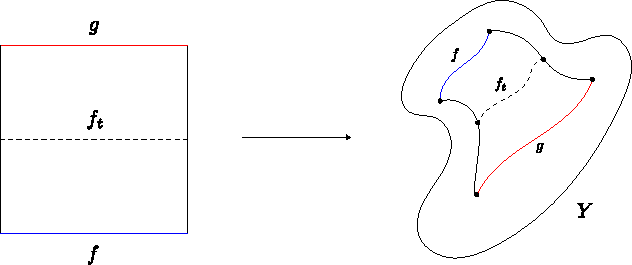
\includegraphics[scale=1]{fig/homotopy.pdf}
\end{figure}

We say that a map is \textbf{nullhomotopic} if it is homotopic to a constant map. Suppose that $f$ and $g$ agree on $A$, then $f$ and $g$ are \textbf{homotopic rel $A$} if there is a homotopy between them that fixes $A$. Note that if $f$ and $g$ agree on $A$ and are homotopic via the straight line homotopy, then they are homotopic rel $A$.

\begin{defn}[]
Two paths $f,g$ are \textbf{path homotopic}, written $f \simeq_p g$, if they are homotopic rel $\left\{ 0,1 \right\}$.
\end{defn}

The \textbf{straight line homotopy} between $f,g:X\to \mathbb{R}^{n}$ is defined
\[
	F(x,t) = (1-t)f(x)+tg(x).
\] 
If $X$ is convex, then the straight line homotopy can be used to show that any two maps (and, by extension, paths) are homotopic.

We can ``multiply" paths $\alpha$ and $\beta$ by first traveling along $\alpha$, then $\beta$, both at double speed. We denote the product of $\alpha$ and $\beta$ by $\alpha\beta$. Note that although this is similar to function composition, we read $\alpha\beta$ left to right instead of right to left.

\begin{prop}
Path multiplication respects path homotopy, i.e. if $\alpha \simeq_p \alpha'$ and $\beta \simeq_p \beta'$, then $\alpha\beta \simeq_{p} \alpha'\beta'$.
\end{prop}
{\color{red}I do this for general homotopies in the next section.}

A \textbf{loop} at $p$ is a path that starts and ends at $p$. Path homotopies easily extend to work with loops instead, since loops are just a special type of path.

\begin{figure}[H]
	\centering
	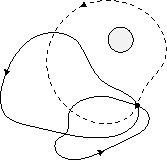
\includegraphics[scale=1.5]{fig/homotopic.pdf}
	\caption{The solid loops are homotopic, but the dashed loop is not homotopic to either of the others because of the hole in the space.}
\end{figure}


%%%%%%%%%%%%%%%%%%%%
% The Fundamental Group
%%%%%%%%%%%%%%%%%%%%

\section{The Fundamental Group}

\begin{lem}
Homotopy and homotopy rel $A$ are both equivalence relations.
\end{lem}

\begin{defn}[]
	The \textbf{fundamental group} of $X$ at $p$ is
	\[
		\pi_1(X,p) \doteq \left\{ [\alpha] \;|\; \alpha \text{ a loop at } p \right\}
	\] 
	with group operation
	$
		[\alpha][\beta] \doteq [\alpha \beta].
	$ 
\end{defn}

Since path multiplication respects path homotopy, the above group operation is well-defined for all representative $\alpha$,$\beta$.

\begin{prop}
	If $p,q$ are in the same path component of $X$, then $\pi_1(X,p) \cong \pi_1(X,q)$.
\end{prop}
\begin{proof}
	There must be a path $\gamma$ from $p$ to $q$, so if $\alpha$ is a loop at $p$, then $\gamma^{-1}\alpha\gamma$ is a loop at $q$. Then it's easy to check that
	\begin{align*}
		\phi:\pi_1(X,p)&\to \pi_1(X,q),\\
		[\alpha]&\mapsto [\gamma^{-1}\alpha\gamma]
	\end{align*}
	is a well-defined homomorphism with homomorphic inverse, i.e. an isomorphism.
\end{proof}

\begin{cor}
If $X$ is path connected, then all points in $X$ have isomorphic fundamental groups.
\end{cor}

\begin{defn}[]
If we have a continuous map $f:(X,x)\to (Y,y)$, then this induces a homomorphism between fundamental groups
\begin{align*}
	f_{*}:\pi_1(X,x)&\to \pi_1(Y,y)\\
	[\alpha]&\mapsto [f\circ \alpha]
\end{align*}
called the \textbf{induced homomorphism} of $f$.
\end{defn}
This being a homomorphism follows from the distributivity of function composition.

\begin{prop}
If $f \simeq f'$ and $g \simeq g'$, then $gf \simeq g'f'$.
\end{prop}
\begin{proof}
If $f \simeq f'$ via $F$ and $g \simeq g'$ via $G$, then the composite map
\[
\begin{tikzcd}
	X\times I\rar{F\times 1_{I}} & Y\times I \rar{G} & Z
\end{tikzcd}
\] 
maps $(x,0) \mapsto (gf)(x)$ and $(x,1)\mapsto (g'f')(x)$.
\end{proof}

\begin{cor}
If $f \simeq g$, then $f_{*}=g_{*}$.
{\color{red}Only works if $f$ and $g$ are homotopic rel endpoints, I think. Otherwise the equivalence classes are in different fundamental groups.}
\end{cor}
\begin{proof}
	Since $f \simeq g$ and $\alpha \simeq \alpha$, we know $f\circ \alpha \simeq g\circ \alpha$, so $f_{*}([\alpha]) = [f\circ \alpha] = [g\circ \alpha]=g_{*}([\alpha])$.
\end{proof}

\begin{prop}
If we have a sequence of continuous maps
\[
	\begin{tikzcd}
		X\rar{f}&Y\rar{g}&Z,
	\end{tikzcd}
\] 
then their induced homomorphisms satisfy $(g\circ f)_{*}=g_{*}\circ f_{*}$.
\end{prop}

\begin{thrm}[]
	If $X \cong Y$, then $\pi_1(X,p) \cong \pi_1(Y,q)$.
\end{thrm}
\begin{proof}
	Suppose $X \cong Y$ via $f$, then we can picture the situation as below.
	\[
	\begin{tikzcd}
		(X,p)\arrow[r,"f",bend left]&(Y,q)\arrow[l,"g=f^{-1}",bend left]
	\end{tikzcd}
	\] 
	These two maps then induce homomorphisms between the fundamental groups.
	\[
        \begin{tikzcd}
                \pi_1(X,p)\arrow[r,"f_{*}",bend left]&\pi_1(Y,q)\arrow[l,"g_{*}",bend left]
        \end{tikzcd}
        \]
	Since $f_{*}g_{*}=(f\circ g)_{*}=(1_{Y})_{*}=1_{\pi_1(X,p)}$ and $g_{*}f_{*}=(1_{X})_{*}=1_{\pi_1(Y,q)}$, the two fundamental groups are isomorphic.
\end{proof}

\begin{prop}
	$\pi_1(X,p) \times \pi_1(Y,q) \cong \pi_1(X\times Y,(p,q))$.
\end{prop}

\begin{defn}[]
	$X$ if \textbf{simply connected} if it is path connected and $\pi_1(X,p)$ is trivial for some $p$ (and thus for all $p$).
\end{defn}

\begin{thrm}[]
	$\pi_1(S^{1})\cong \mathbb{Z}$.
\end{thrm}

\begin{thrm}[Brouwer Fixed Point]
	If $X \cong D^{2}$ (the closed unit disk), then every continuous map $f:X\to X$ has a fixed point.
\end{thrm}


%%%%%%%%%%%%%%%%%%%%
% Covering Spaces
%%%%%%%%%%%%%%%%%%%%

\section{Covering Spaces}

\begin{defn}[]
	A \textbf{covering space} of $B$ is a space $E$ and a \textbf{covering map} $p:E\to B$. For all $x \in B$, there is a neighborhood $U$ of $x$ such that $p^{-1}(U)$ is a disjoint union of homeomorphic copies of $U$. Such neighborhoods are called \textbf{evenly covered}.
\end{defn}
Equivalently, a covering space of is a fiber bundle with discrete fibers. Note that $p$ must be continuous and surjective.

This is more about open sets than points. Once we get $U$ from $x$, we forget about $x$ in the definition.

{\color{red}Figure.}

\begin{ex}[]
	$\mathbb{R}$ is a covering space of $S^{1}$. One possible covering map is
		\begin{align*}
			p:\mathbb{R}&\to S^{1}\\
			t&\mapsto (\cos 2\pi t,\sin 2\pi t).
		\end{align*}
\end{ex}

\begin{defn}[]
If $p:E\to B$ is a covering map and $f:X\to B$ is continuous, then we say that $\tilde{f}$ \textbf{lifts} $f$ if $p \circ \tilde{f}=f$.
\[
\begin{tikzcd}
	&E\dar{p}\\
	X\rar{f}\arrow[ur,"\tilde{f}"]&B
\end{tikzcd}
\] 
\end{defn}

\begin{prop}
Covering maps are open.
\end{prop}

\begin{cor}
Covering maps are quotient maps.
\end{cor}
{\color{red}The converse isn't necessarily true.}

We can lift homotopies (and by extension, more specific maps like paths) to a covering space. Since an evenly covered neighborhood can contain multiple copies of an open set in the base space, though, we need to specify the starting point in order to make the lift unique.

\begin{thrm}[Homotopy Lifting Extension Property]
	Fix a homotopy $F:X \times I\to B$ and suppose $F|_{X \times \left\{ 0 \right\}}$ has a lift $f$. Then there is a unique lift $\tilde{F}$ of $F$ that extends $f$.
\[
\begin{tikzcd}
	X\rar{f}\arrow[d,"1_{X}\times 0"']&E\dar{p}\\
	X\times I\rar{F}\arrow[ur,dashed,"\exists ! \; \tilde{F}"]&B
\end{tikzcd}
\] 
\end{thrm}
This is saying that if we fix what happens at $t=0$ in the lift, then the lift is unique.

\begin{cor}[Path Lifting Lemma]
	A path $\gamma$ in $B$ has a unique lift $\tilde{\gamma}$ if we fix $\tilde{\gamma}(0)$.
	\[
	\begin{tikzcd}
		&E\dar{p}\\
		I\arrow[ur,dashed,"\tilde{\gamma}"]\rar{\gamma}&B
	\end{tikzcd}
	\] 
\end{cor}

\begin{cor}[Path Homotopy Lifting Lemma]
	Suppose $\gamma_1,\gamma_2$ are paths in $B$ that both start at $x$. Let $F$ be a path homotopy between them rel $x$. If we specify some $\tilde{x} \in p^{-1}(x)$ and fix a lift $f$ of $F|_{I \times \left\{ 0 \right\}}$, then there is a unique lift of $F$ rel $\tilde{x}$, that extends $f$.
	\[
	\begin{tikzcd}
		I\arrow[d,"1_{I}\times 0"']\rar{f}&E\dar{p}\\
		I\times I\rar{F}\arrow[ur,dashed,"\exists ! \; \tilde{F}"]&B
	\end{tikzcd}
	\] 
\end{cor}

%%%%%%%%%%%%%%%%%%%%
% The Borsuk-Ulam Theorem
%%%%%%%%%%%%%%%%%%%%

\section{The Borsuk-Ulam Theorem}

\begin{thrm}[]
	Suppose $X=A \cup B$ with $A,B$ path connected and open and $A \cap B$ path connected. If $i_{A}$ and $i_{B}$ are the usual inclusion maps, then for all $[\gamma] \in \pi_1(X,x)$, we can decompose it into
	\[
		[\gamma] = [\alpha_1] \cdots [\alpha_{k}],
	\] where each $[a_i]$ lies either in $i_{A_*}(\pi_1(A,x))$ or $i_{B_{*}}(\pi_1(B,x))$.
\end{thrm}

\begin{cor}
If $n \geq 2$, then $S^{n}$ is simply connected.
\end{cor}
\begin{proof}
	$(S^{n}-\left\{ \text{a point} \right\}) \cong \mathbb{R}^{n}$ by stereographic projection. Define $U$ to be $S^{n}$ minus the north pole and $V$ to be $S^{n}$ minus the south pole. Then $U,V \cong \mathbb{R}^{n}$, so
	\[
		\pi_1(U), \pi_1(V) \cong \pi_1(\mathbb{R}^{n}) \cong \left\{ e \right\}.
	\] Since $n \geq 2$, $U \cap V$ is path connected. Then by the previous theorem, we can decompose any $[\gamma] \in \pi_1(S^{n})$ into the product of trivial equivalence classes, so $[\gamma]=[e]$. Thus $\pi_1(S^{n})$ is trivial and $S^{n}$ is subsequently simply connected.
\end{proof}

\begin{cor}
	You cannot cover $S^{n}$ with $n+1$ antipode-free (doesn't contain antipodal points) closed sets.
\end{cor}
\begin{proof}
	Suppose $\left\{ A_i \right\}_{i=1}^{n+1}$ are closed and cover $S^{n}$. Let $d_i:S^{n}\to \mathbb{R}$ be the distance to $A_{i}$, i.e.
	\[
		d_i(x) = \inf_{y \in A_{i}}{\Vert{x-y}\Vert}.
	\] This is continuous, so
	\begin{align*}
		f:S^{n}&\to \mathbb{R}^{n}\\
		x&\mapsto (d_1(x), \dots, d_{n}(x))
	\end{align*}
	is also continuous. Then by Borsuk-Ulam, $f(x)=f(-x)$ for some $x \in S^{n}$. This implies $d_{i}(x)=d_{i}(-x)$ for all $i$. If $d_i(x)=d_i(-x)=0$ for some $i$, then $x,-x$ are both limit points of $A_i$. Since $A_i$ is closed, though, $x,-x \in A_i$. If none of the $d_i(x)$ are 0, then $x,-x \not\in A_i$ for $1 \leq i \leq n$, which forces $x,-x \in A_{n+1}$.
\end{proof}

\begin{thrm}[Borsuk-Ulam]
	Every continuous map $f:S^{n}\to \mathbb{R}^{n}$ satisfies $f(x)=f(-x)$ for some $x \in S^{n}$.
\end{thrm}

\begin{cor}
	If $Y \cong \mathbb{R}^{n}$, then every continuous map $f:S^{n}\to Y$ satisfies $f(x)=f(-x)$ for some $x \in S^{n}$.
\end{cor}
\begin{proof}
	The situation is depicted below.
	\[
	\begin{tikzcd}
		S^{n}\rar{f}&Y\rar[bend left]{g}&\mathbb{R}^{n}\lar[bend left]{g^{-1}}
	\end{tikzcd}
\] The composition $gf$ is a continuous map $S^{n}\to \mathbb{R}^{n}$, so we can apply Borsuk-Ulam to find a point $x \in S^{n}$ such that $(gf)(x)=(gf)(-x)$. But this is also a fixed point of $f$, as
\[
	f(x) = g^{-1}(gf(x)) = g^{-1}(gf(-x)) = f(-x).
\] 
\end{proof}

%%%%%%%%%%%%%%%%%%%%
% Homotopy Type
%%%%%%%%%%%%%%%%%%%%

\section{Homotopy Type}

A homeomorphism $f:X\to Y$ is a map satisfying $f \circ f^{-1}=1_{Y}$ and $f^{-1} \circ f=1_{X}$. We can loosen this restriction to gain the notion of a homotopy equivalence.

\begin{defn}[]
	A \textbf{homotopy equivalence} $f:X\to Y$ is a map satisfying
\begin{align*}
	f \circ f^{-1} &\simeq 1_{Y},\\
	f^{-1} \circ f &\simeq 1_{X}.
\end{align*}
We say that two spaces $X$ and $Y$ are \textbf{homotopy equivalent} or have the same \textbf{homotopy type} if we can find a homotopy equivalence between them. We denote this by $X \simeq Y$.
\end{defn}

\begin{prop}
	If $f,g:X\to Y$ are homotopic with induced maps $f_{*},g_{*}$ on $\pi_1(X,p)$, then
	\[
		\pi_1(Y,f(p)) \cong \pi_1(Y,g(p))
	\] via an isomorphism $\hat{\gamma}$ satisfying $\hat{\gamma}f_{*}=g_{*}$.
\[
\begin{tikzcd}
	\pi_1(X,p)\rar{f_{*}}\arrow[dr,"g_{*}"]&\pi_1(Y,f(p))\dar[dashed]{\hat{\gamma}}\\
			     &\pi_1(Y,g(p))
\end{tikzcd}
\] 
\end{prop}
\begin{proof}
	Suppose $f \simeq g$ via $F$, then $\gamma(t) \doteq F(p,t)$ is path from $f(p)$ to $g(p)$. Then
	\[
		\hat{\gamma}([\alpha]) \doteq [\gamma^{-1} \cdot \alpha \cdot \gamma]
	\] is an isomorphism between $\pi_1(Y,f(p))$ and $\pi_1(Y,g(p))$. {\color{red}Show $\hat{\gamma}f_{*}=g_{*}$.}
\end{proof}

\begin{prop}
	If $X \simeq Y$ via $f$, then $\pi_1(X,p)\cong \pi_1(Y,f(p))$.
\end{prop}
\begin{proof}
	Suppose
	\[
        \begin{tikzcd}
                (X,p)\arrow[r,"f",bend left]&(Y,q)\arrow[l,"g",bend left]
        \end{tikzcd}
        \]
	where $fg \simeq 1_{Y}$ and $gf \simeq 1_{X}$. Then since homotopic maps have the same induced homomorphisms, $f_{*}g_{*}=(fg)_{*}=(1_{Y})_{*}$ and $g_{*}f_{*}=(gf)_{*}=(1_{X})_{*}$, so the two fundamental groups are isomorphic.
\end{proof}
This shows that all we need for fundamental groups to be isomorphic is for the original spaces to be homotopic. The earlier result when the original spaces were homeomorphic is then a special case of this.

When working with homotopy type, entire spaces can behave like single points. These are exactly the spaces whose identity maps are nullhomotopic.

\begin{defn}[]
A space $X$ is \textbf{contractible} if $1_{X}$ is nullhomotopic.
\end{defn}

\begin{prop}
A space is contractible if and only if it has the homotopy type of a one-point space.
\end{prop}


%%%%%%%%%%%%%%%%%%%%
% Deformation Retracts
%%%%%%%%%%%%%%%%%%%%

\section{Deformation Retracts}

\begin{defn}[]
	Suppose $A \subset X$. A \textbf{retraction} of $X$ onto $A$ is a map $r:X\to A$ that fixes $A$. If $i:A\hookrightarrow X$ is the usual inclusion map, then this means $r\circ i = 1_{A}$. We call $A$ a \textbf{retract} of $X$.

	A \textbf{deformation retraction} of $X$ onto $A$ is a map $F:X\times I \to X$ such that
	\begin{align*}
		F(x,0)&=x,\\
		F(a,t)&=a \quad \forall t,\\
		F(x,1)&\in A.
	\end{align*}
	We call $A$ a \textbf{deformation retract} of $X$.
\end{defn}
Suppose $i:A\hookrightarrow X$ is the usual inclusion, then a retraction satisfies $r \circ i = 1_{A}$.

Note that $F$ is a homotopy rel $A$ between $1_{X}$ and $i \circ r$, where $r:X\to A$ is some retraction of $X$ onto $A$. Thus an equivalent definition of a deformation retract is that there is some retraction $r$ of $X$ onto $A$ such that $i \circ r \simeq 1_{X}$.

Retractions take a space and teleport it onto a subset of itself in a continuous way. Deformation retractions have an added time component: they make the space flow onto a subset of itself in a continuous way.

Deformation retracts are useful because they let you crush part of a space without changing its homotopy type.

\begin{prop}
	If $A$ is a deformation retract of $X$, then $A \simeq X$.
\end{prop}
\begin{proof}
	Since $A$ is a deformation retract of $X$, then there's some retract $r:X\to A$ such that $i \circ r \simeq 1_{X}$. Since $r$ is a retract, it must satisfy $r \circ i = 1_{A}$.
\end{proof}

Note that this isn't necessarily true for ordinary retracts. Take any non-contractible space $X$ (like a sphere) and map everything to one point (call this subset $Y$). Since this map is constant, it's continuous and, subsequently, a retraction. But since $X$ wasn't contractible and any map $f:Y\to X$ is constant, there's no function $g:X\to Y$ such that $fg \simeq 1_{X}$. Thus $X$ and $Y$ can't have the same homotopy type.


\end{document}
